{\bf Version \#0.1}: These lecture notes are intended to be a concise source of reading material for \school{} students taking \emph{\course{}} (ME4XX) in the fall semester of 2021. Students are encouraged to follow the numerous links to external resources. During this semester students were expected to develop a parallel finite difference solver for linear advection equation from scratch using C, OpenMP, and MPI.
% During this semester students were expected to develop a parallel k-means data clustering algorithm from scratch using C, OpenMP, and MPI.

\begin{figure}[h]
\begin{center}
 \begin{subfigure}{0.3\textwidth}
  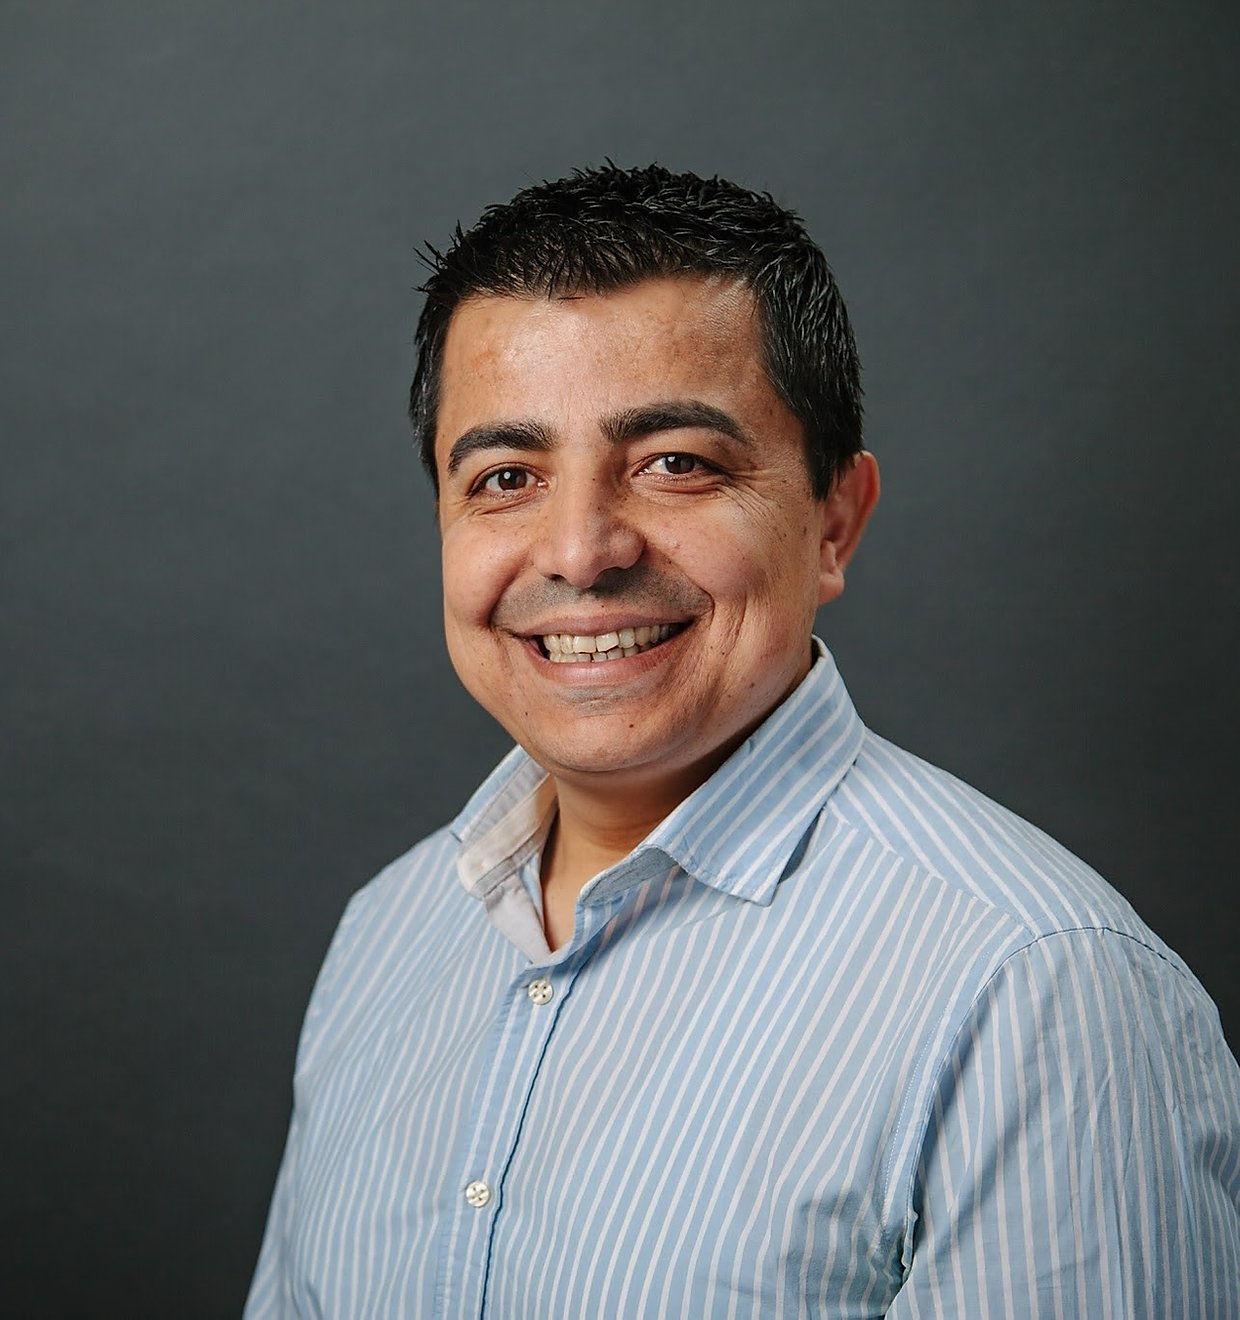
\includegraphics[width=0.99\textwidth]{figures/cover/ali.jpg}
  \caption{}
 \end{subfigure}
 \begin{subfigure}{0.3\textwidth}
  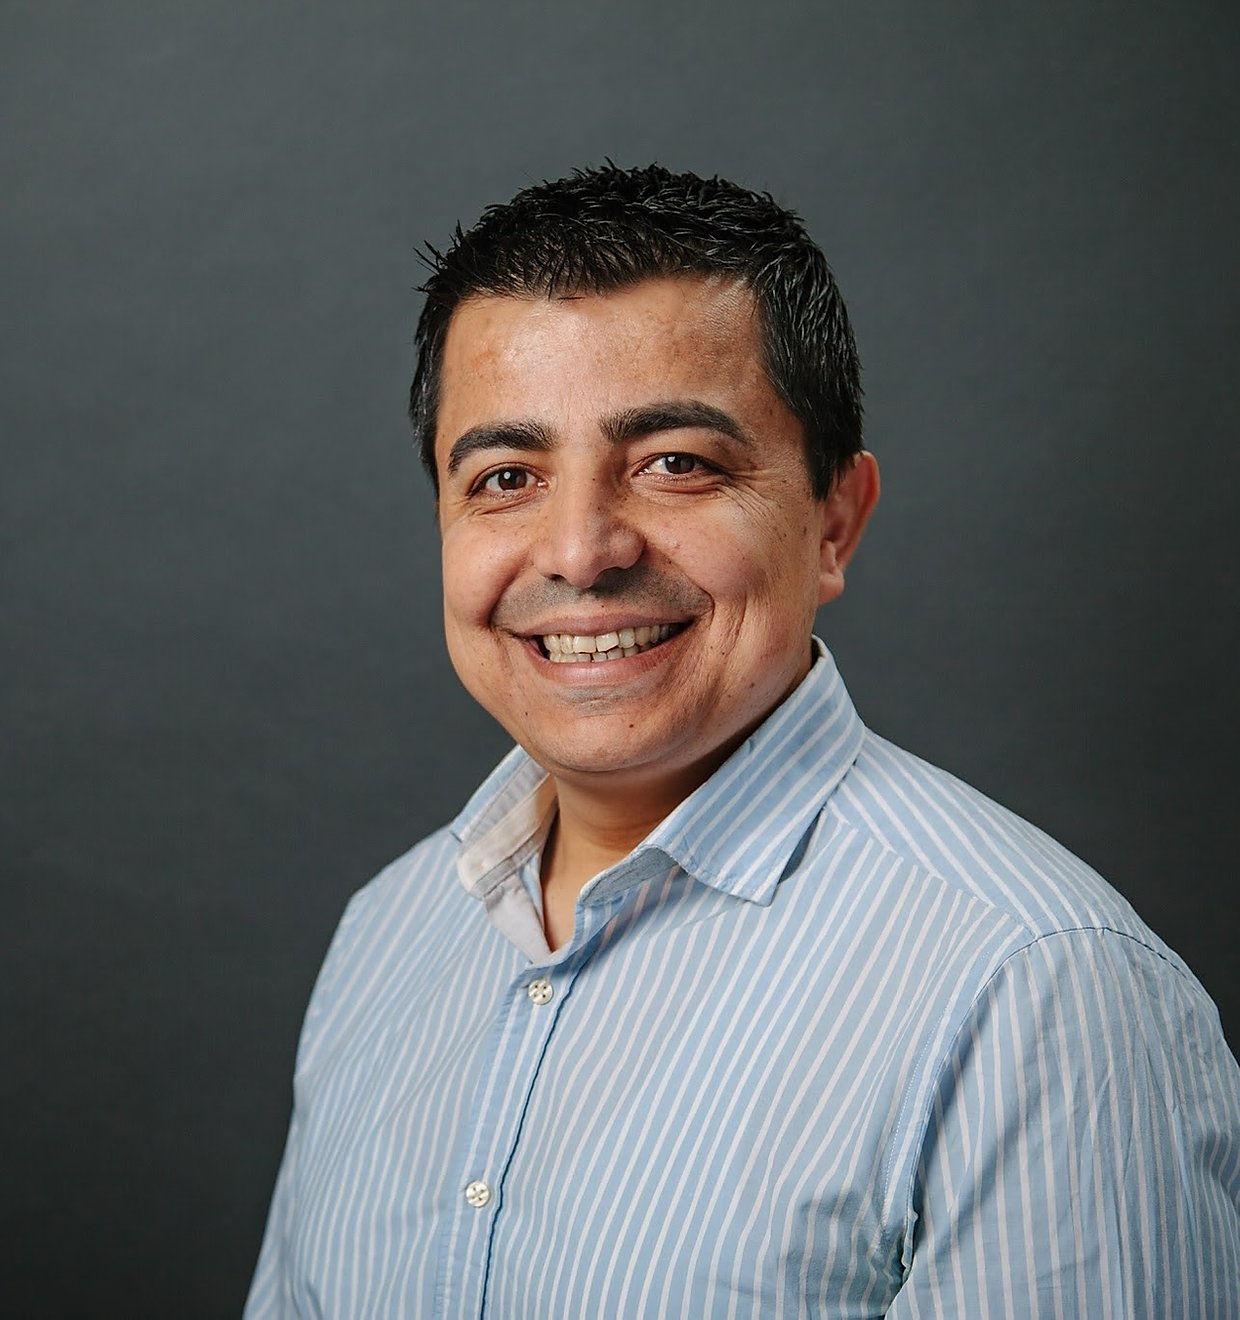
\includegraphics[width=0.99\textwidth]{figures/cover/ali.jpg}
  \caption{}
 \end{subfigure}
 \\
 \begin{subfigure}{0.3\textwidth}
  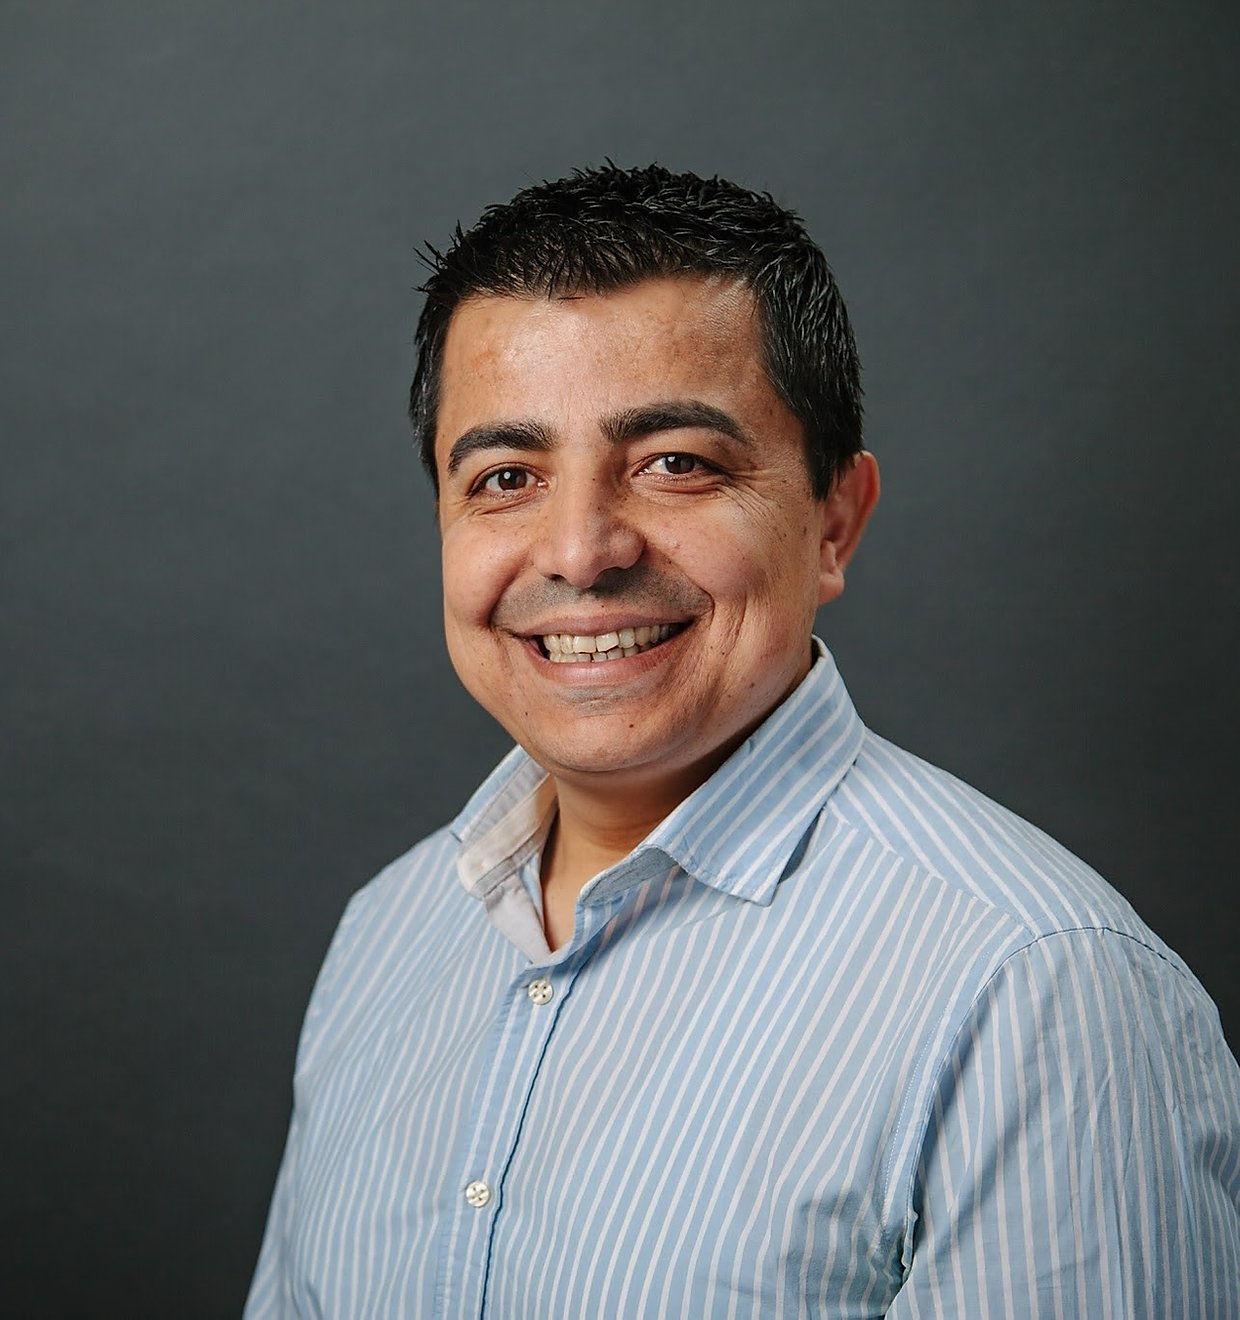
\includegraphics[width=0.99\textwidth]{figures/cover/ali.jpg}
  \caption{}
 \end{subfigure}
 \begin{subfigure}{0.3\textwidth}
  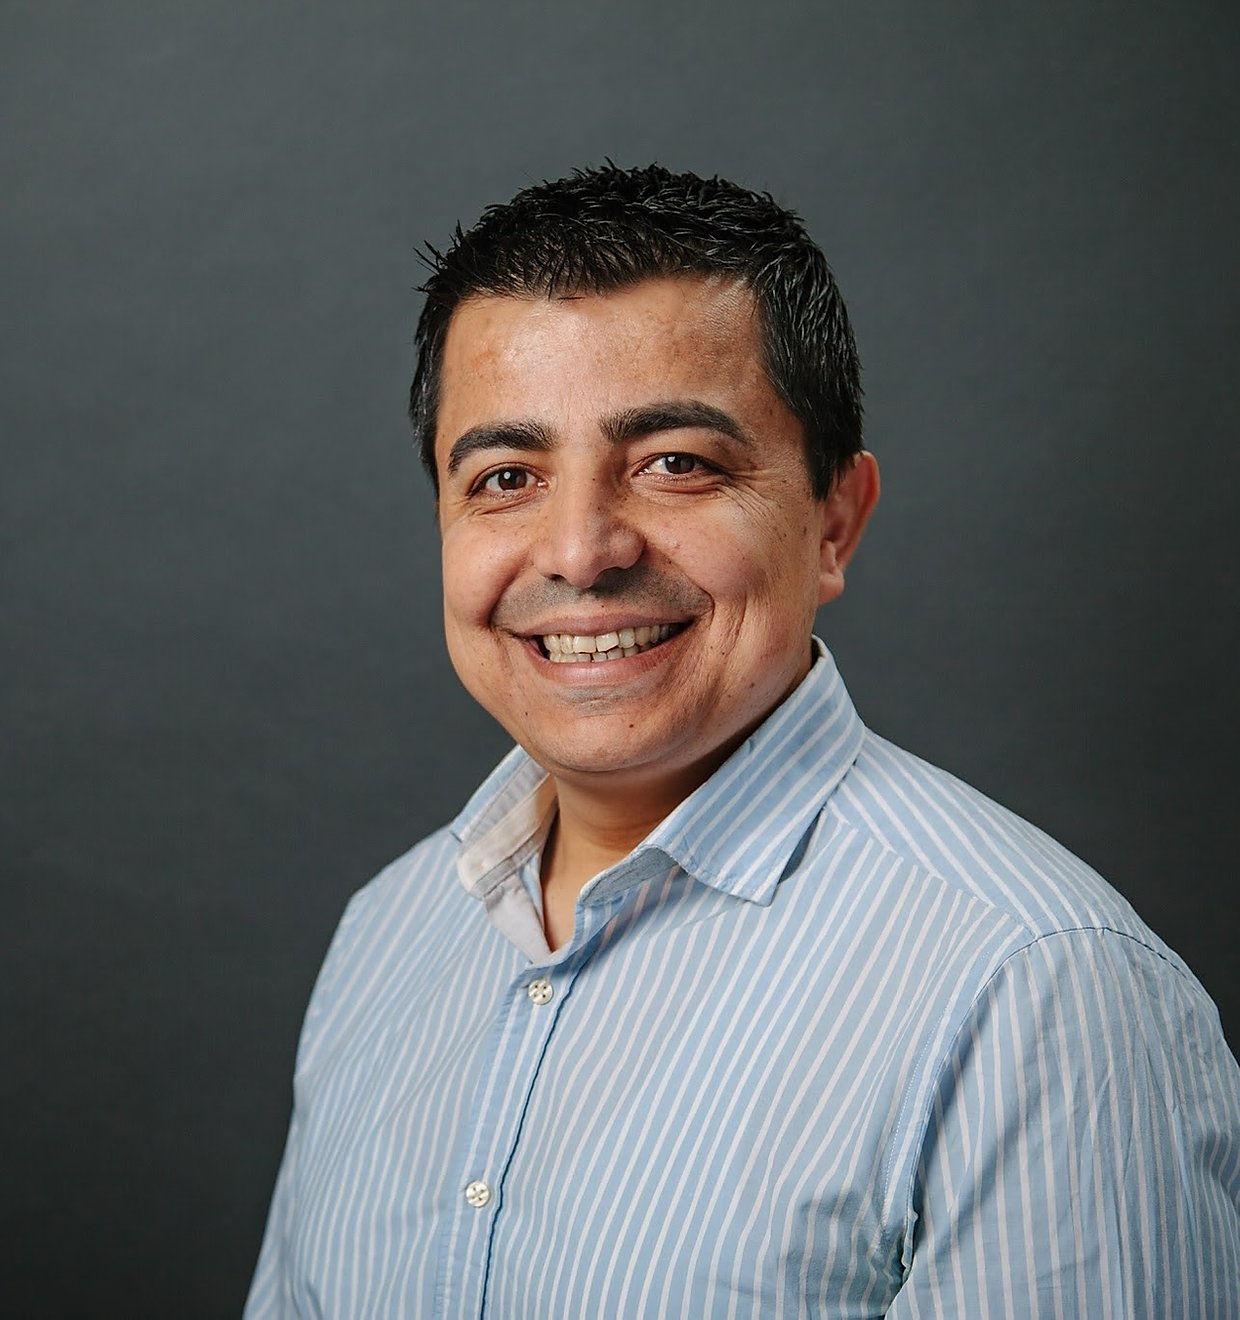
\includegraphics[width=0.99\textwidth]{figures/cover/ali.jpg}
  \caption{}
 \end{subfigure}
 \begin{subfigure}{0.3\textwidth}
  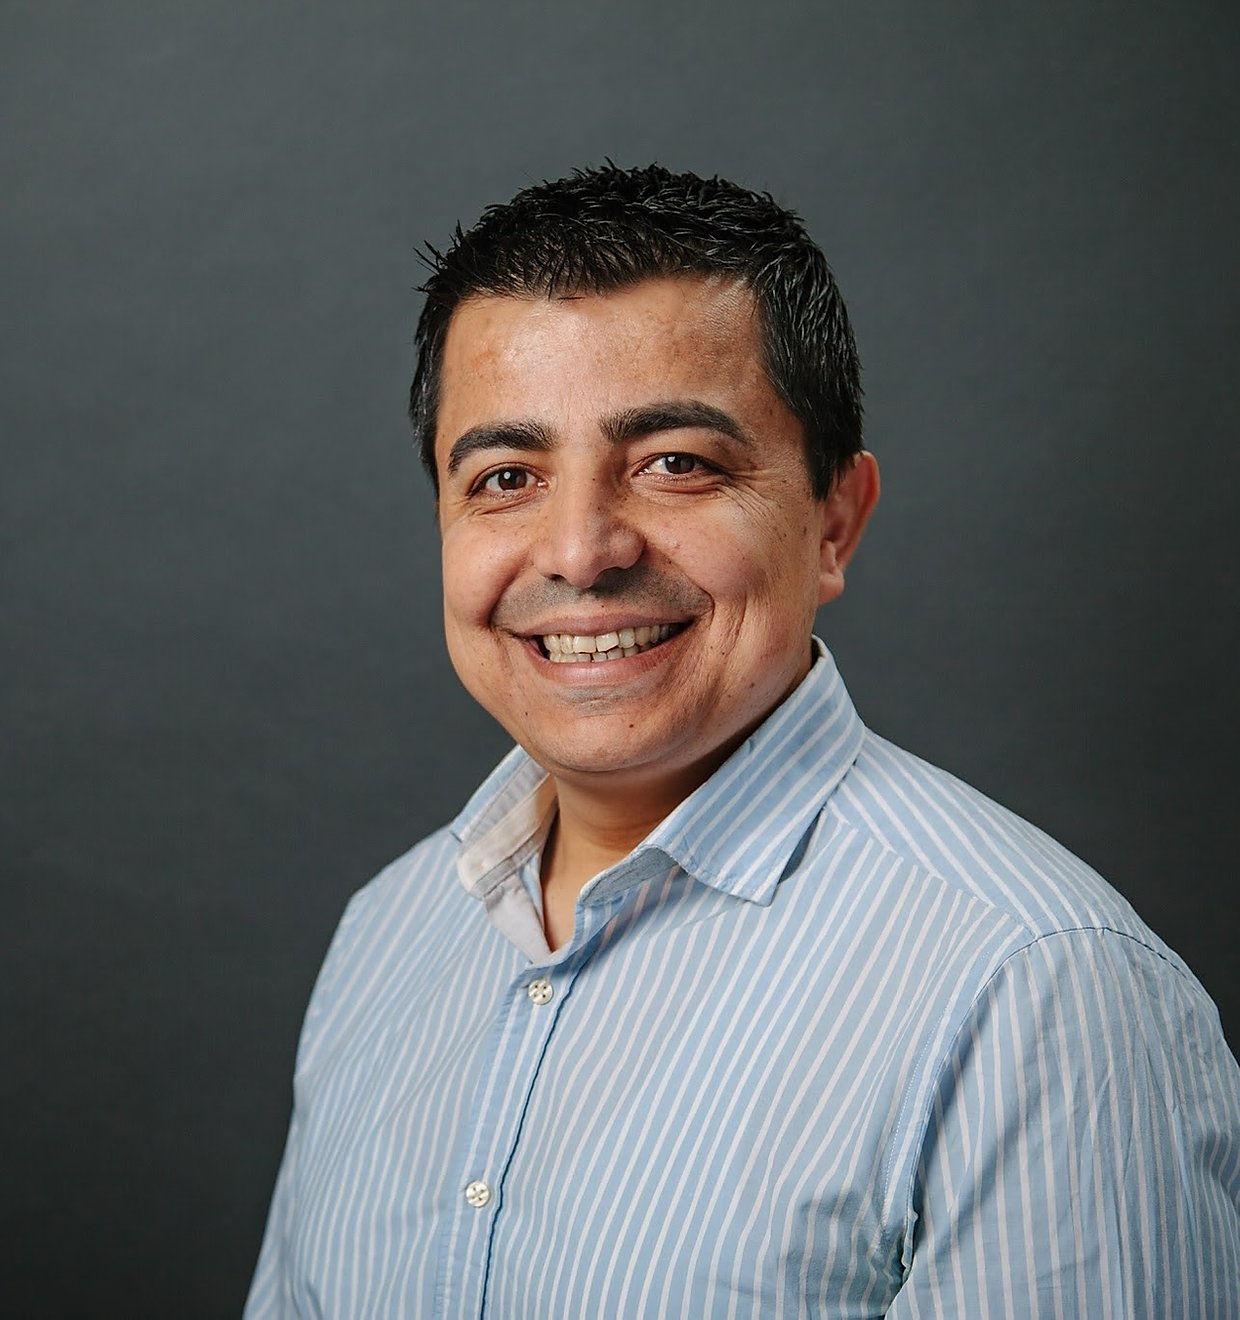
\includegraphics[width=0.99\textwidth]{figures/cover/ali.jpg}
  \caption{}
 \end{subfigure}
\caption{a) Tim Warburton, Professor @ VT b) Ali Karakus, Professor @ METU c) Noel Chalmers, Scientist @ AMD Research d) Anthony Austin, Professor @ NPS d) Kasia \'{S}wirydowicz, Scientist @ NREL }
\label{fig:SquareCylinder2DSubcycle}
\end{center}
\end{figure}



% \begin{figure}[htbp]
% \begin{center}
% 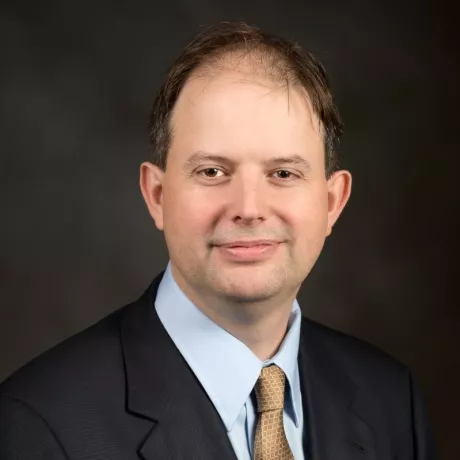
\includegraphics[width=.45\textwidth]{figures/cover/tim.jpg}\\
% 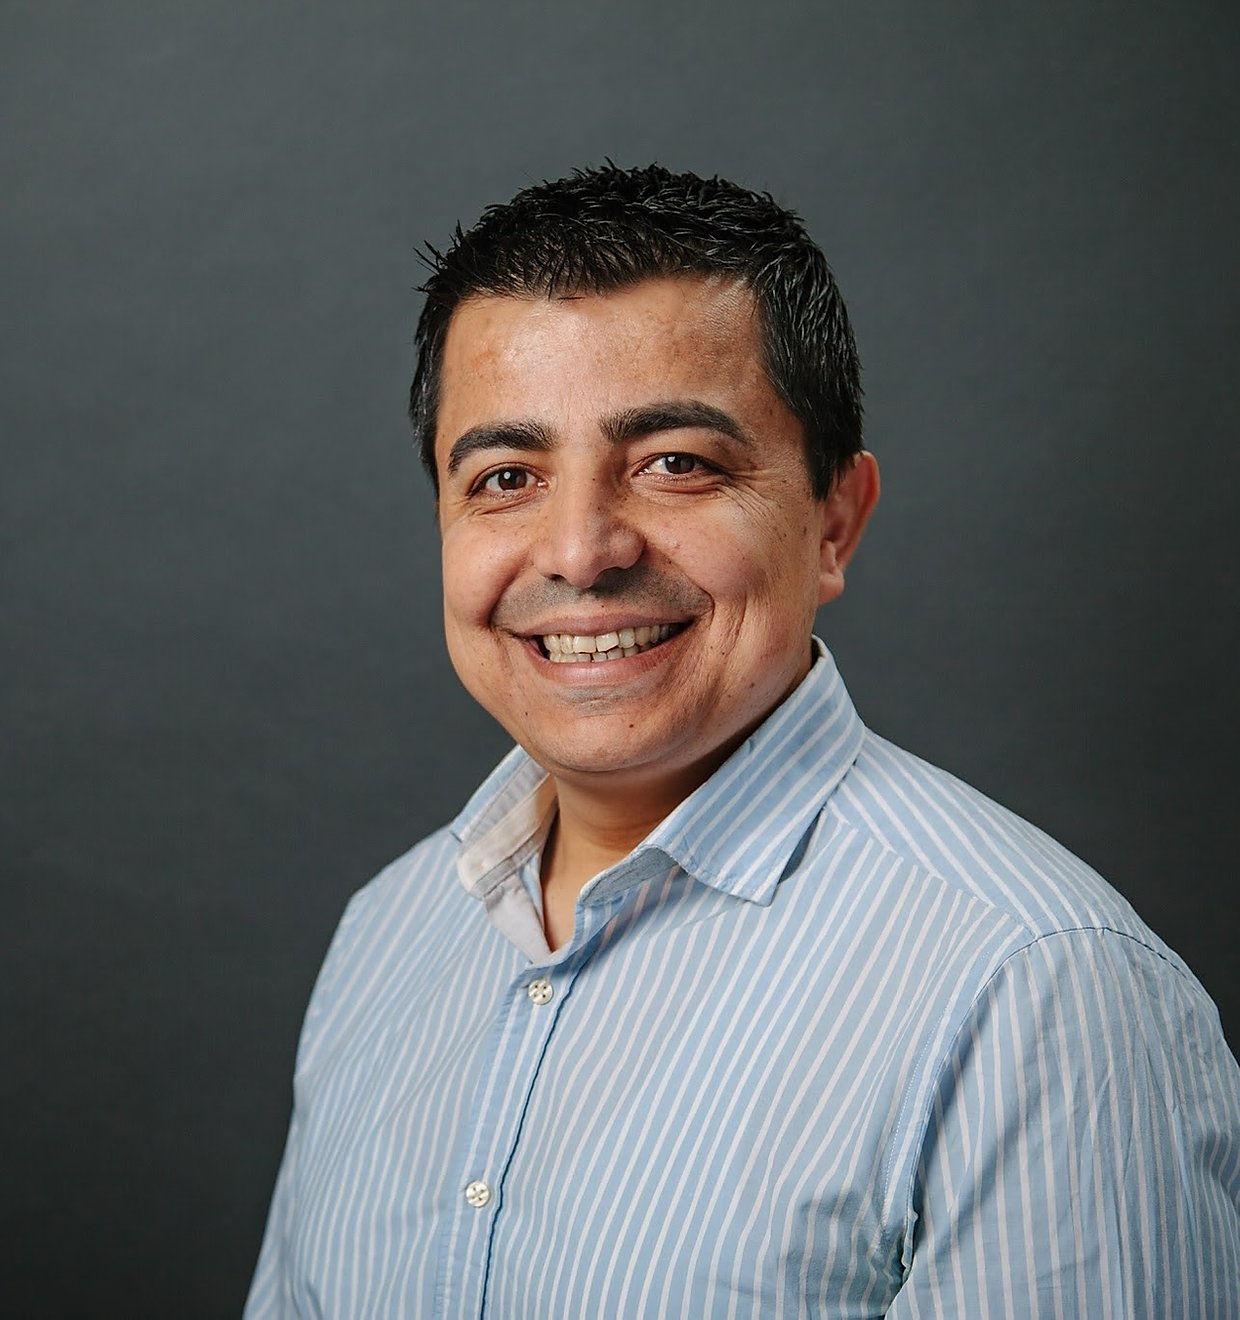
\includegraphics[width=.45\textwidth]{figures/cover/ali.jpg}
% \end{center}
% \end{figure}

We gratefully acknowledge the contributions to these notes from Anthony Austin, Noel Chalmers and Kasia \'{S}wirydowicz. 

\autha{} and \authb{}, \semester{}.